\textbf{With 16 animals nothing changed.} All three widths learned every fact, although there
is now four times as much to know about each animal.

\textbf{With 256 animals no model learned everything.} Widths 16 and 32 ended flat at a score
of 37. PENDING-REPEAT2. Width 8 was still rising slowly when its 40 minutes ran out, at a score
of 59, so it is not finished and I cannot say how far it would have gone
(figure \ref{fig:round32}).

\begin{figure}[H]
\centering
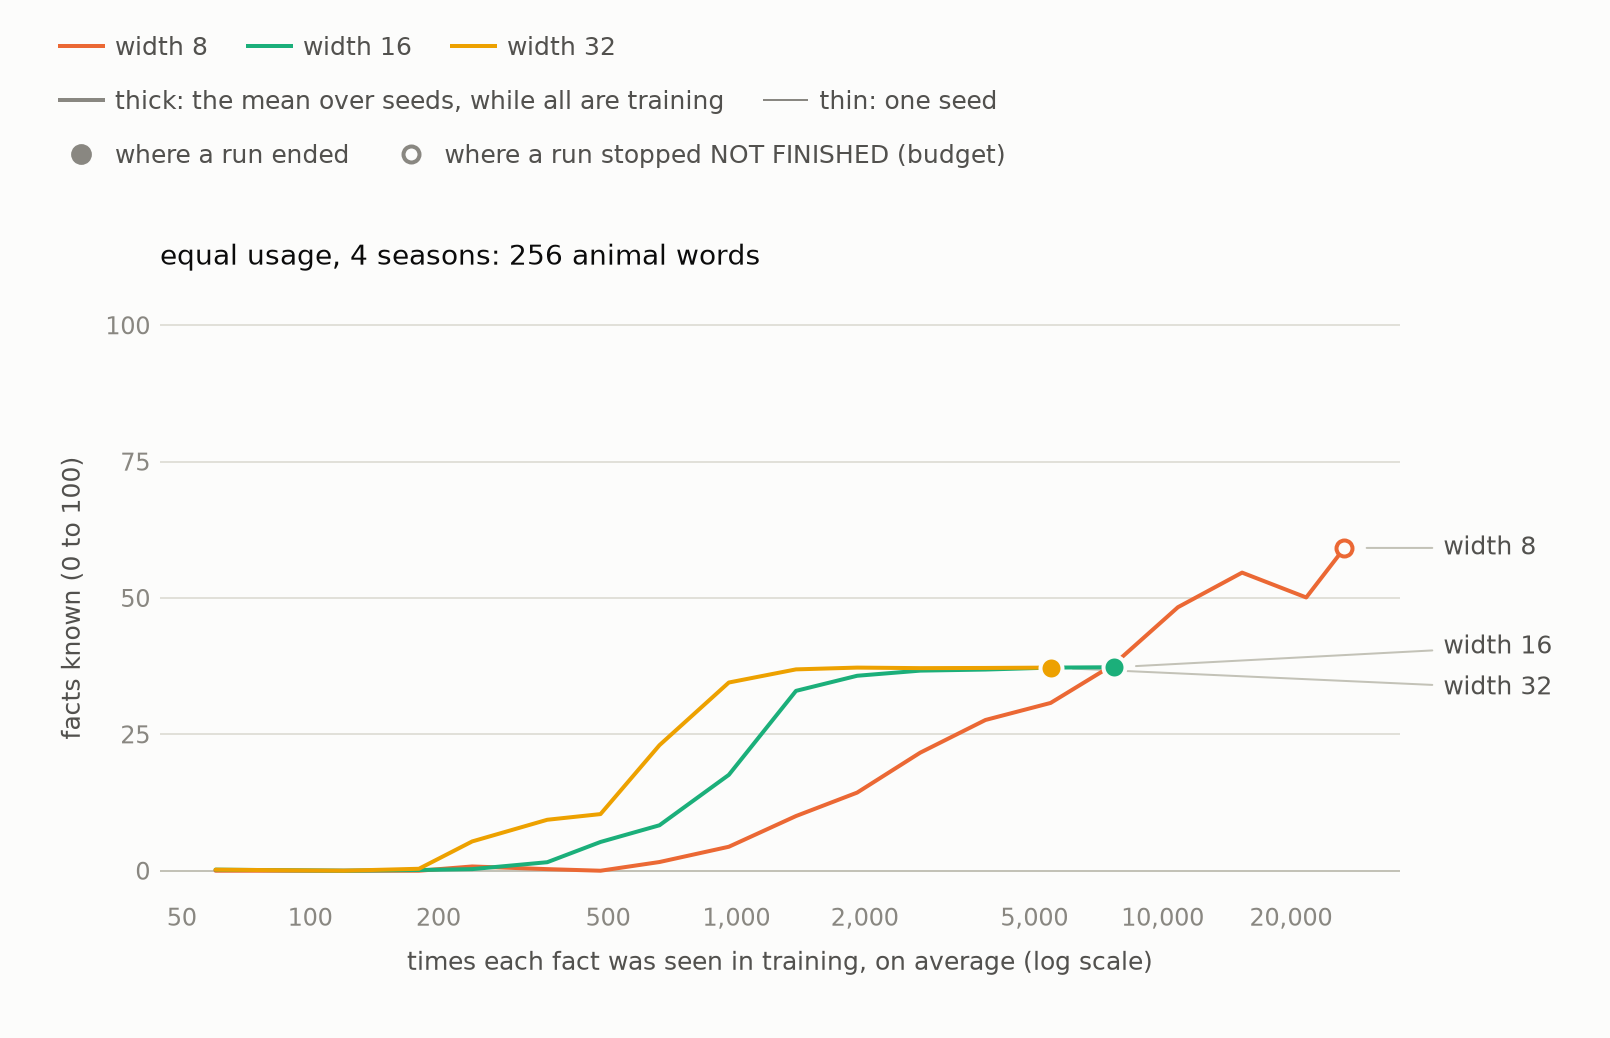
\includegraphics[width=0.62\textwidth]{figures/learning_equal_x4.png}
\caption{The models on 256 animals with 32 bits each, as training went on. The two wider
models rise quickly and then stop at 37. The narrowest rises slowly and passes them. A hollow
dot marks a run that was not finished.}
\label{fig:round32}
\end{figure}

This is the first time in the experiment that more words made a model worse. For width 16,
conditions (a) and (b) of our rule hold: it scores 100 on 16 animals and ends flat at 37 on
256. But condition (c) fails. The model twice as wide does not score higher; it scores the
same 37. By our agreement that means something other than size is holding width 16 back. The
right half of table \ref{tab:round32} agrees: if they had learned all 256 animals, width 16
would have been about one-third full and width 32 about one-tenth full. The two models that
stopped were not short of room.

\textbf{What stopped them: they ignore the season.} A score of 37 is 53 facts in 100 right
(remember that 0 on our score already stands for 25 in 100). It is also exactly what a model
scores if it takes no notice of the season word. Take one animal and one kind of fact, say
what foxes eat. The right answer differs from season to season. The two models that stopped
name the same food for all four seasons, and they do so for 99\% of the animals and kinds of
fact (table \ref{tab:season}). The food they name is always the one that is right in more
seasons than any other. They have learned what each animal is \emph{usually} like, and nothing
more. On 16 animals the same two widths did learn the seasons.

\begin{table}[H]
\centering\small
\begin{tabular}{@{}rrrr@{}}
\toprule
Width & Repeat & Facts known & Same value given \\
 & & & in all four seasons \\
\midrule
8 & 1 & 59* & 5\% \\
16 & 1 & 37$^{\dagger}$ & 99\% \\
32 & 1 & 37$^{\dagger}$ & 99\% \\
\bottomrule
\end{tabular}

\caption{The models on 256 animals with 32 bits each. Last column: for how many animals and
kinds of fact the model names the same value in all four seasons. A model that knew every fact
would do so for about 2\%. A dagger marks a run that ended flat, a star one that was not
finished.}
\label{tab:season}
\end{table}

Width 8 did learn to use the season on 256 animals, which is how it got past 37. I do not know
why the narrowest model learned this and the two wider ones did not.

\textbf{Does the stand-still ever end?} Section \ref{sec:round1} showed that a model can stand
still for a long time and then move again. PENDING-LONGRUN.

\textbf{What this round says about size.} Less than its heading might suggest. Lack of room
was not what stopped widths 16 and 32, and a bigger model did not help. That is all. It does
not show that size never matters. The one model that the rough guide says was nearly full,
width 8 on 256 animals (85\%), was still improving when it was stopped. And the round changed
two things at once. Each animal had four times as much to be remembered. And no fact could be
answered from the animal word alone any more: the model had to put the animal and the season
together. These runs cannot tell me which of the two made 256 animals so much harder than 16.
